% !TeX encoding = UTF-8
% !TeX spellcheck = fr_FR


\definecolor{couleurbackintr}{HTML}{7F00FF}
\definecolor{couleurtextintr}{HTML}{FFFFFF}
\definecolor{couleurbackfonc}{HTML}{C780FF}
\definecolor{couleurtext}{HTML}{000000}
\definecolor{couleurbackextr}{HTML}{DDB3FF}
\begin{figure}[htp]
	\centering
	\tikzset{
		basic/.style={draw, rounded corners=2pt, thick, text width=8em, align=flush center, text=couleurtext, node distance=2em, anchor=center},
		intrant/.style={basic, fill=couleurbackintr, text=couleurtextintr},
		fonction/.style={basic, fill=couleurbackfonc},
		extrant/.style={basic, fill=couleurbackextr}
	}
	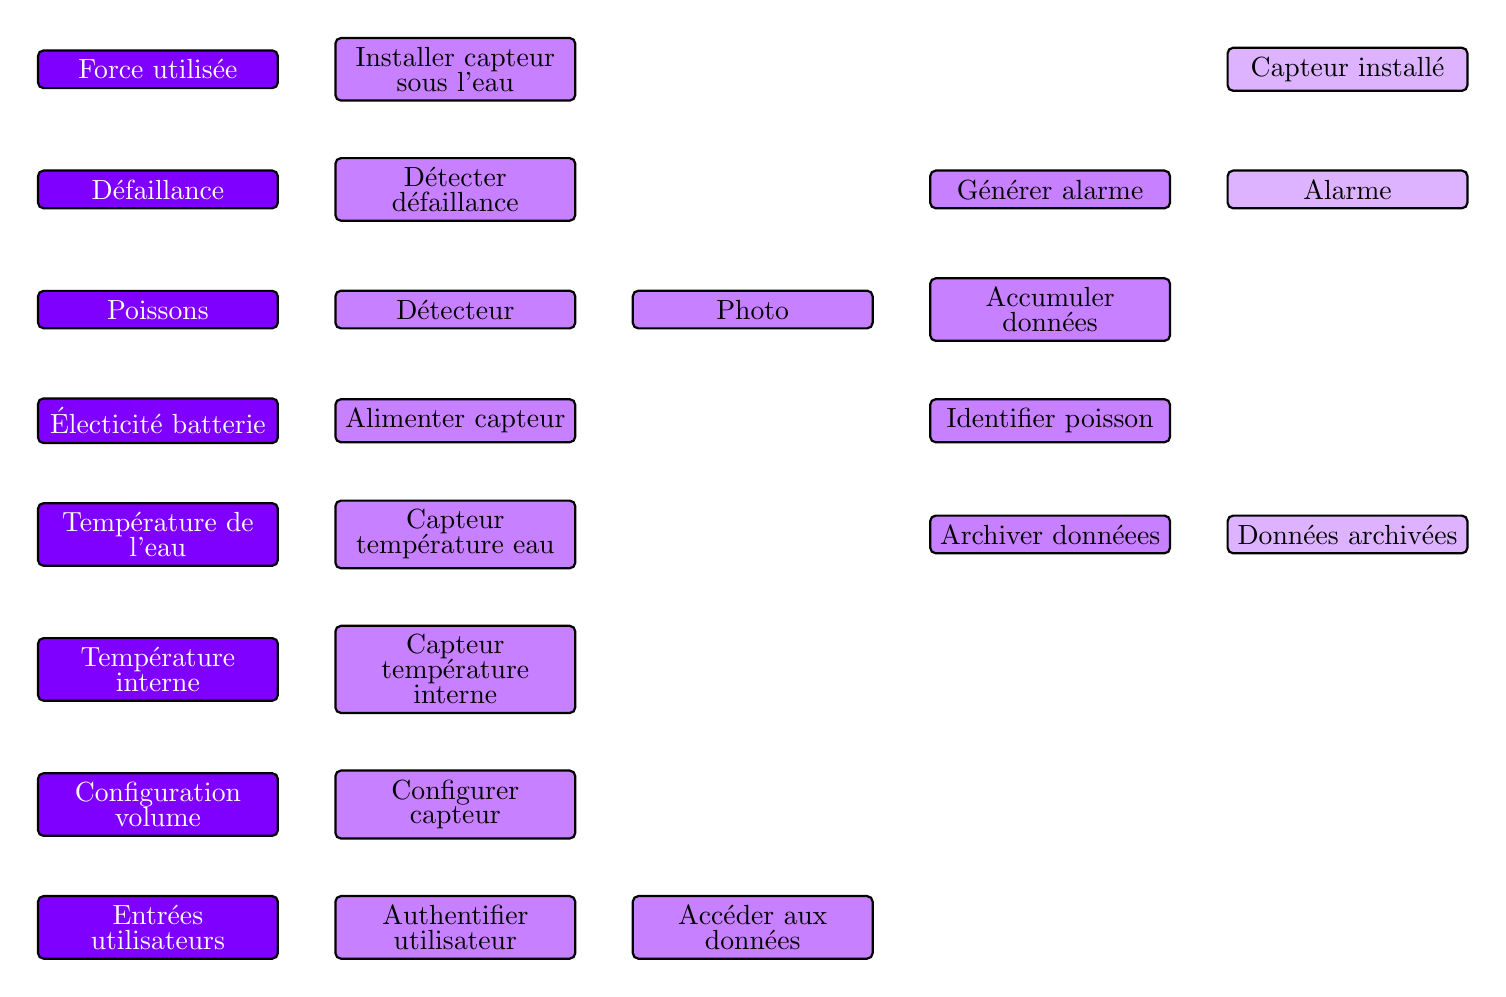
\begin{tikzpicture}[]
		\fontsize{10}{9} \selectfont
		% intrants
		\matrix[row sep=2em, column sep=2em] {
			% 1re ligne
			%TODO changer nom
			\node[intrant](forcutil){Force utilisée}; & \node[fonction](instcapt){Installer capteur sous l'eau}; & & & \node[extrant](captinst){Capteur installé}; \\
			% 2me ligne
			\node[intrant](defailla){Défaillance}; & \node[fonction](detcdefa){Détecter défaillance}; & & \node[fonction](genralrm){Générer alarme}; & \node[extrant](alarme){Alarme}; \\
			\node[intrant](poissons){Poissons}; & \node[fonction](detecteu){Détecteur}; & \node[fonction](photo){Photo}; & \node[fonction](accudonn){Accumuler données}; & \\
			\node[intrant](elecbatt){Électicité batterie}; & \node[fonction](alimcapt){Alimenter capteur}; & & \node[fonction](idenpois){Identifier poisson}; & \\
			\node[intrant](tempreau){Température de l'eau}; & \node[fonction](captteau){Capteur température eau}; & & \node[fonction](archdonn){Archiver donnéees}; & \node[extrant](donnarch){Données archivées}; \\
			\node[intrant](tempintr){Température interne}; & \node[fonction](capttcpt){Capteur température interne}; & & & \\
			\node[intrant](confvolm){Configuration volume}; & \node[fonction](confcapt){Configurer capteur}; & & & \\
			\node[intrant](entrutil){Entrées utilisateurs}; & \node[fonction](authutil){Authentifier utilisateur}; & \node[fonction](accedonn){Accéder aux données}; & & \\
		};
	\end{tikzpicture}
	\caption{Diagramme fonctionnel}
	\label{f:caf_diag_fonc}
\end{figure}